\documentclass[basic,plain]{inVerba-notes}

\newcommand{\userName}{Cullyn Newman}
\newcommand{\class}{BI:\@ 428}
\newcommand{\theTitle}{Midterm Corrections}
\newcommand{\institution}{Portland State University}

\begin{document}
    
\section{Week 2: Chromosomes}
\begin{itemize}
    \minor{\item[1-B] Original question: Explain this phenomenon, specifically what happens, when it happens and how it relates to nondisjunction.
    
    Your critique: ``Exact causes of nondisjunction = any possibilities (there is one associated with the MAE) (only 1/2 pt off)''

    Original relevant response: \dots The coexistence of a normal cell with an aneuploid line can allow the for the development of trisomy, which would otherwise would not survive early on. Exact causes of nondisjunction is not known, but it does appear to be most common in the first meiotic division in females. This is why MAE is a suspected factor, since the chances of nondisjunction probably increased due to errors accumulated with age\dots}

    \textbf{Somewhat revised response:} ``Exact causes'' does not equal ``any possibilities''---it means there is more than one. There is an association with advanced maternal age and increased risk of nondisjunction, particularly due to the prolonged meiotic arrest of human oocytes~\cite{eichenlaub2013oocyte}, but that does not mean there is an exact cause.

    Personal remark: I didn't do this correction for the points, but I did specify that nondisjunction increase due to errors accumulated with age. It seems silly to lose any points over this in the first place unless you were asking for the specific mechanism by which age increases risk, but that seems like a stretch.

    \minimal{\item[1-D.] Original question: Discuss one of the three autosomal trisomies that makes it to birth. What is the phenotype associated with that chromosomal abnormality?

    Your critique: ``asked for the phenotype as well (some included frequency and survival) (worth 3 pts)''

    Original relevant portion of response: \dots  This is also why most cases of down syndrome (specifically trisomy 21, the most common trisomy) have two maternal and one paternal chromosomes, giving it three copies of chromosome 21 (karyotype 47,XX,+21/47,XY,+21).}

    \textbf{Revised response:} Trisomy 21, the most common trisomy and commonly known as Down syndrome, has many phenotypic affects, with most displaying a variety of physical and intellectual disabilities. Those affected have characteristic facial features (low muscle tone, flattened nose, slanted eyes, and more), stunted growth, epilepsy, various mental disorders, and often congenital heart defects. The most frequent abnormality is mental impairment roughly equal to those of 8 years olds that affects nearly all cases.
    
    \newpage 

    \minor{\item[4.] Original question: a. What is constitutive heterochromatin?\\
    b. where is it found?\\
    c. What banding technique demonstrates these areas the best?
    
    
    You critique: Although there are other areas of constitutive heterochromatin than the telomeres, they are not scattered throughout--\\
    - many responses included what the basic C-banding technique did (which is)\\
    - many responses included the type of repeats often seen (such as)
    
    
    Original response: Constitutive heterochromatin are regions of DNA found throughout the chromosome of eukaryotes. They are found in telomeres and scattered throughout the chromosome, but mostly in the pericentromeric (near the centromere) regions of chromosomes. The is much more in chromosomes 1,9,16, 19, and Y. 

    Visualization is done by using the C-banding technique, which is stains regions of DNA\@. Since constitutive heterochromatin are so condensed, then it is usually very easy to identify them due to darker staining.

    Constitutive heterochromatin mostly consist of various repeats, accounting for about 6.5\% of the human genome. Typically, they do not have many genes, but some have been found. It is thought that histone modifications are one of the main ways of condensing constitutive heterochromatin, which suggests they play a role in some heritable characteristics due to epigenetics.}

    \textbf{Revised Response}: Okay, this one I feel like I totally answered what was asked in my original response. \\A: I descried what it did, briefly discussed repeats, how staining is used. \\B: Definitely described where they were found. \\C: ableit this was brief, I did state how staining was used to identify them due to their condensed nature.
    
    I'm not sure where I lost points, since the question did not ask for types of repeats, or what C-banding techinque did in great detail. 
    
    Was it due to the scattered bit? Because it is true. Constitutive heterochromatin are found in other areas other than pericentromeric regions and telomeres.~\cite{saksouk2015constitutive}. 

    \begin{center}
        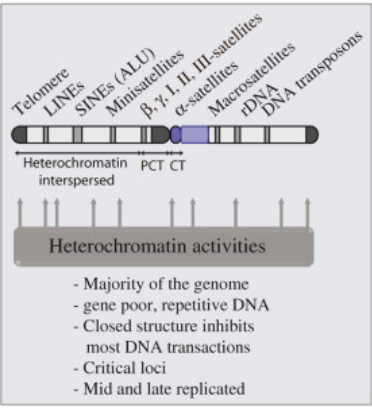
\includegraphics[scale=0.5]{images/midterm-correct.png}
    \end{center}

    So yeah, okay, not ``scattered randomly''. But I'm not writing a review paper here, and I didn't explictly say randomly; scattered here meant: ``found at different loci along the chromosome'' which is stated in figure 1 of reference paper I used. I also literally specified, in the same sentence, ``\dots but mostly in the pericentromeric (near the centromere) regions of chromosomes.

    \minor{\item[5.] Original question: Look up and describe the process of comparative genomic hybridization.
    b. Give an example of its use.

    Your critique: ``Asks you to describe the CGH technique.'' 

    Original relevant response: CGH is a molecular cytogenetic (branch of genetics relating chromosomes to behavior) method used to quickly and efficient compare two genomic DNA samples (control and reference) in order to detect deletions or duplications. CGH is only able to detect unbalanced chromosomal abnormalities, since it compares copy number variants to relative ploidy levels. However, it still can lead to identification of candidate genes.

    There are multiple methods, such as FISH (fluorescence in situ hybridization), blocking, DNA labelling, CGH arrays, and others, all of which are applied in a wide variety of techniques with different advantage.}

    \textbf{Revised response}: I feel like I did describe it, but since you still provided barely any feedback, then I must assume you mean to describe the \textit{method} of CGH\@. So here is an example of one some basic method: 

    Test and reference DNA samples are isolated then fragmented into small segments. Nick translation (using DNA polymerase I) is used then used to label DNA\@. Simultaneous hybridization are labeled DNA samples are then mixed together with DNA oligonucleotides bound to a microarray. A fluorescence microscope with various filters is used to detect the hybridized DNAs sequences. Yellow = balanced DNA; Excess due to duplication = red; Green = excess reference due to DNA deletion.
\end{itemize}

\section{Week 3: Sexual Development}
\begin{itemize}
    \item Original question: b. What is the purpose of this phenomenon?
    
    Your critique: Missing b.

    Original response: I did not state purpose.

    \textbf{Revised Response}: The purpose of the bar body is to inactive an X chromosome in cells with more than one. Conflicting interactions between various genes could be a problem when the cells had two copies of X chromosomes. The condensed cells are essential for proper gene regulation by allowing just one set of genes to be expressed.
\end{itemize}


\bibliographystyle{apacite}
\bibliography{midterm.bib}
\end{document}